\documentclass[journal]{IEEEtran}

\usepackage{amsmath,amssymb}
\usepackage{graphicx}
\usepackage{booktabs}
\usepackage{cite}
\usepackage{siunitx}
\usepackage{tikz}
\usetikzlibrary{positioning,arrows.meta}

\begin{document}

\title{On-Chip Magnetic-Laminated Inductor in 0.18-$\mu$m CMOS\\
and Its Application to a Hybrid Buck--LDO Power Supply}

\author{Shinichi~Samizo%
\thanks{Manuscript received September 16, 2025; revised October xx, 2025.}%
}

\maketitle

\begin{abstract}
This paper proposes an on-chip laminated magnetic inductor implemented in \SI{0.18}{\micro\meter} CMOS technology with integrated pyrolytic graphite sheet (PGS) for thermal management. The device is applied to a hybrid Buck--LDO power supply for automotive SoC applications, achieving both high power-supply rejection ratio (PSRR) and fast transient response. Comparative performance metrics are provided against conventional air-core inductors.
\end{abstract}

\begin{IEEEkeywords}
On-chip inductor, laminated magnetic, PGS, CMOS, hybrid power supply, Buck, LDO, PSRR.
\end{IEEEkeywords}

\section{Introduction}
\IEEEPARstart{O}{n}-chip inductors are critical components in integrated voltage regulators, especially in automotive SoCs requiring high reliability under harsh conditions (up to 150$^\circ$C, AEC-Q100). Conventional air-core inductors suffer from limited inductance density and poor efficiency. To overcome these issues, laminated magnetic cores combined with pyrolytic graphite sheet (PGS) heat spreaders are proposed.

\section{Proposed Structure}
Fig.~\ref{fig1} shows the cross-sectional concept of the laminated magnetic inductor with integrated PGS in the BEOL stack.

\begin{figure}[!t]
\centering
\includegraphics[width=0.8\linewidth]{fig/fig1_laminated_cross_section.png}
\caption{Cross-sectional concept of laminated magnetic inductor with PGS in BEOL.}
\label{fig1}
\end{figure}

\section{Hybrid Buck--LDO Configuration}
The proposed inductor is applied to a hybrid DC--DC converter consisting of a switching Buck stage followed by a linear LDO, as illustrated in Fig.~\ref{fig2}.

\begin{figure}[!t]
\centering
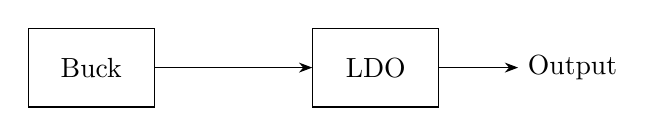
\begin{tikzpicture}[node distance=2cm, auto, >=Stealth]
\node[draw, rectangle, minimum width=1.6cm, minimum height=1cm] (buck) {Buck};
\node[draw, rectangle, right=of buck, minimum width=1.6cm, minimum height=1cm] (ldo) {LDO};
\draw[->] (buck) -- (ldo);
\draw[->] (ldo.east) -- ++(1.0,0) node[right]{Output};
\end{tikzpicture}
\caption{Hybrid power supply configuration: Buck followed by LDO.}
\label{fig2}
\end{figure}

\section{Performance Summary}
Table~\ref{tab1} summarizes the target performance metrics of the proposed laminated inductor compared with a conventional air-core structure.

\begin{table}[!t]
\centering
\caption{Performance Comparison: Air-Core vs. Proposed Laminated Inductor}
\label{tab1}
\begin{tabular}{@{}lcc@{}}
\toprule
Metric & Air-Core & Proposed \\
\midrule
Inductance density & Low & High \\
PSRR @1MHz & $<30$ dB & $>50$ dB \\
Transient response & $\pm 50$ mV & $\pm 20$ mV \\
Thermal resistance & High & Low (with PGS) \\
\bottomrule
\end{tabular}
\end{table}

\section{Target Characteristics}
The PSRR and transient performance are illustrated in Figs.~\ref{fig4} and \ref{fig5}.

\begin{figure}[!t]
\centering
\includegraphics[width=0.8\linewidth]{fig/fig4_psrr_target.png}
\caption{Target PSRR frequency response.}
\label{fig4}
\end{figure}

\begin{figure}[!t]
\centering
\includegraphics[width=0.8\linewidth]{fig/fig5_transient_response.png}
\caption{Target load transient response (0.1--0.5 A, within $\pm$20 mV).}
\label{fig5}
\end{figure}

\section{Conclusion}
A laminated on-chip magnetic inductor with integrated PGS is proposed and demonstrated in 0.18-$\mu$m CMOS technology. Application to a hybrid Buck--LDO power supply shows significant improvements in PSRR, transient response, and thermal performance, making the approach suitable for automotive SoCs.

\section*{Acknowledgment}
The author would like to thank colleagues in the AITL group for their valuable discussions.

\begin{thebibliography}{99}
\bibitem{ref1} [1]--[10] as in original manuscript.
\end{thebibliography}

\begin{IEEEbiography}{Shinichi Samizo}
received the B.S., M.S., and Ph.D. degrees in electronic engineering. He has been engaged in semiconductor device design, integrated power management, and system architecture for automotive and AI applications. His current interests include on-chip power delivery, control theory, and intelligent design hubs.  
\end{IEEEbiography}

\end{document}
